%%%%%%%%%%%%%%%%%%%%%%%%%%%%%%%%%%%%%%%%%
% Journal Article
% LaTeX Template
% Version 1.4 (15/5/16)
%
% This template has been downloaded from:
% http://www.LaTeXTemplates.com
%
% Original author:
% Frits Wenneker (http://www.howtotex.com) with extensive modifications by
% Vel (vel@LaTeXTemplates.com)
%
% License:
% CC BY-NC-SA 3.0 (http://creativecommons.org/licenses/by-nc-sa/3.0/)
%
%%%%%%%%%%%%%%%%%%%%%%%%%%%%%%%%%%%%%%%%%

%----------------------------------------------------------------------------------------
%	PACKAGES AND OTHER DOCUMENT CONFIGURATIONS
%----------------------------------------------------------------------------------------

\documentclass[twoside,twocolumn]{article}

%\usepackage{booktabs,caption}
\usepackage[flushleft]{threeparttable}
\usepackage{graphicx}
\usepackage{blindtext} % Package to generate dummy text throughout this template 

\usepackage[sc]{mathpazo} % Use the Palatino font
\usepackage[T1]{fontenc} % Use 8-bit encoding that has 256 glyphs
\linespread{1.05} % Line spacing - Palatino needs more space between lines
\usepackage{microtype} % Slightly tweak font spacing for aesthetics

\usepackage[english]{babel} % Language hyphenation and typographical rules

\usepackage[hmarginratio=1:1,top=32mm,columnsep=20pt, left= 2.35cm, right = 2.35cm, footskip = 2cm]{geometry} % Document margins
\usepackage[hang, small,labelfont=bf,up,textfont=it,up]{caption} % Custom captions under/above floats in tables or figures
\usepackage{booktabs} % Horizontal rules in tables
\usepackage{float}
\usepackage{lettrine} % The lettrine is the first enlarged letter at the beginning of the text
\usepackage{algpseudocode} %for pseudocode
\usepackage{enumitem} % Customized lists
\setlist[itemize]{noitemsep} % Make itemize lists more compact

\usepackage{abstract} % Allows abstract customization
\renewcommand{\abstractnamefont}{\normalfont\bfseries} % Set the "Abstract" text to bold
\renewcommand{\abstracttextfont}{\normalfont\small\itshape} % Set the abstract itself to small italic text

\usepackage{titlesec} % Allows customization of titles
\renewcommand\thesection{\Roman{section}} % Roman numerals for the sections
\renewcommand\thesubsection{\roman{subsection}} % roman numerals for subsections
\titleformat{\section}[block]{\large\scshape\centering}{\thesection.}{1em}{} % Change the look of the section titles
\titleformat{\subsection}[block]{\large}{\thesubsection.}{1em}{} % Change the look of the section titles

\usepackage{fancyhdr} % Headers and footers
\pagestyle{fancy} % All pages have headers and footers
\fancyhead{} % Blank out the default header
\fancyfoot{} % Blank out the default footer
%\fancyhead[C]{Running title $\bullet$ May 2016 $\bullet$ Vol. XXI, No. 1} % Custom header text
\fancyfoot[RO,RE]{\thepage} % Custom footer text

\usepackage{titling} % Customizing the title section

\usepackage{hyperref} % For hyperlinks in the PDF

%----------------------------------------------------------------------------------------
%	TITLE SECTION
%----------------------------------------------------------------------------------------

\setlength{\droptitle}{-4\baselineskip} % Move the title up

\pretitle{\begin{center}\huge\bfseries} % Article title formatting
\posttitle{\end{center}} % Article title closing formatting
\title{Model for the solar system using ordinary differential equations } % Article title

\author{%
\textsc{Andreas Fagerheim}\thanks{\url{https://github.com/AndreasFagerheim/Project-4}} \\[1ex] % Your name
\normalsize Department of Physics, University of Oslo, Norway \\ % Your institution
%\normalsize \href{mailto:john@smith.com}{john@smith.com} % Your email address
%\and % Uncomment if 2 authors are required, duplicate these 4 lines if more
%\textsc{Jane Smith}\thanks{Corresponding author} \\[1ex] % Second author's name
%\normalsize University of Utah \\ % Second author's institution
%\normalsize \href{mailto:jane@smith.com}{jane@smith.com} % Second author's email address
}
\date{\today} % Leave empty to omit a date

%---------------------------------------------------------------------------------------
\renewcommand{\maketitlehookd}{%
\begin{abstract}

This article constructs a model for simulating the solar system. The Forward Euler and velocity Verlot methods will be used to solve the ordinary differential equations that describes the system. Taking an object oriented approach to implementation of the code makes for an more affordable task of expanding the system.


\end{abstract}
}

%----------------------------------------------------------------------------------------

\begin{document}
\maketitle

\section{Introduction}
This article focus on how to solve coupled ordinary differential equations with Euler Forward and velocity Verlet. With these two we will simulate the solar system and look further on the stablety of the two different methods. Further the aim is to develop a structured code which is object oriented for an easier way of creating the desired system we want to simulate.
The system modelled is only affected by the gravitational force between the planets. For this we use Newton's law of gravitation given by:
\begin{equation}
F_G=\frac{GM_{\odot}M_{\mathrm{Earth}}}{r^2}
\end{equation}
%------------------------------------------------
\section{Theory}

\subsection{Escape velocity}
It is interesting looking at what the velocity of earth has to be for it to leave its orbit around the sun. This happens when the potential energy equals the kinetic energy. This leads to the equation;
\begin{equation}
0.5M_1v_{escape}^2 = G\frac{M_1M_2}{r}
\end{equation}
\begin{equation}
v_{escape}= \sqrt{\frac{2GM}{r}} 
\end{equation}
For a system consisting of just the sun and Earth the Earth's escape velocity will be:
\begin{equation}
v_{escape}= \sqrt{\frac{2(4\pi^2 (AU^3/year^2))}{1 (AU)}} = 2\pi \sqrt{2} (AU/year)
\end{equation}
%------------------------------------------------
%------------------------------------------------
\section{Algorithms}
The methods for integrating the system has it offspring from Taulor expansion of functions. 
\[
f(x+h) = f(x) +h\frac{df}{dx}(x)+\frac{1}{2!}\frac{d^2f}{dx^2}(x) +..
\]
One of the methods (Euler Forward) make use of the two first terms in the Taylor expansion while Velocity Verlet uses three terms. 
\subsection{Euler Forward algorithm}
Euler Forward then defines the approximation for next value to be
\begin{equation}
\vec{  x_{i+1}} = \vec{x_{i}} + h \vec{v_i}
\end{equation}
and
\begin{equation}
\vec{  v_{i+1}} = \vec{v_{i}} + h \vec{a_i}
\end{equation}

\begin{algorithmic}[H]

\For {i= 0,1,.., n-1}
\State find $a$ from forces
\State then compute velocity and position
\State $\vec{  x_{i+1}} = \vec{x_{i}} + h \vec{v_i}$
\State $\vec{  v_{i+1}} = \vec{v_{i}} + h \vec{a_i}$
\EndFor
\end{algorithmic}
By using this algorithm the calculation consist of 4 FLOPS (2 in each calculation of next velocity and position). The error is $O(h^2)$ for both $ \vec{  x_{i+1}}$ and $\vec{  x_{i+1}}$. Euler Forward can therefore be said to trade of its low cost in nedd of power for calculations (4 FLOPS) for a lower precision.

\subsection{Verlet method}
Velocity Verlet make use of three terms, as earlier stated;
\begin{equation}\label{eq:verlet1}
 x_{i+1} =x_{i}+ h x_{i}^{(1)} +\frac{h^2}{2} x_{i}^{(2)} + O(h^3)
\end{equation}
and
\begin{equation} \label{eq:verlet2}
v_{i+1} =v_{i}+ h v_{i}^{(1)}+\frac{h^2}{2} v_{i}^{(2)} + O(h^3)
\end{equation}
Here we know all values except the second derivative of the velocity. By Taylor expansion of the first derivative of velocity:

\[
v_{i+1}^{(1)} =v_{i}^{(1)}+ h v_{i}^{(2)} + O(h^2)
\] 
\[
hv_{i}^{(2)} \approx v_{i+1}^{(1)}-  v_{i}^{(1)}
\] 
Using this and we can rewrite equations \ref{eq:verlet1} and \ref{eq:verlet2} containing only known values;
\begin{equation}
x_{i+1} =x_{i}+ h v_{i} +\frac{h^2}{2} v_{i}^{(1)} + O(h^3)
\end{equation}
and
\begin{equation}
v_{i+1} =v_{i}+ \frac{h}{2} \left( v_{i+1}^{(1)}+v_{i}^{(1)} \right)+ O(h^3)
\end{equation}
Due to $v_{i+1}^{(1)}$ being dependent on $x_{i+1}$ calculating position at updated time ($t_{i+1}$) is necessary for calculating the new velocity.WE also know that $v_{i}^{(1)} = a_i $. In pseudo code this will look somthing like the figure below.
\begin{algorithmic}[H]
\For {i= 0,1,.., n-1}
\State find $a$ from forces
\State then compute velocity and position
\State $\vec{  x_{i+1}} = \vec{x_{i}} + h \vec{v_i}+\frac{h^2}{2}\vec{a_i}$
\State $\vec{  v_{i+1}} = \vec{v_{i}} + \frac{h}{2} (\vec{a_{i+1}}+\vec{a_i})$
\EndFor
This algorithm has 9 FLOPS in its calculation (5 FLOPS for position and 4 FLOPS for velocity). The strenght of the method is instead its local error witch is in order $O(h^3)$.
\end{algorithmic}

\subsection{Object oriented}
The code is structured with with classes after a straightforward approach. To do this there is implemented three different classes to make up our system. The first class is the class Univers which sets up the system we want to simulate with its bodies and natural laws they have to obey. This urges the class Legemer (Bodies) which holds the attributes of bodies. Last is the class Intregrand wich implements to the two different methods for integration.

%------------------------------------------------
%------------------------------------------------

\section{Results}
\textbf{Figure} \textbf{1} and \textbf{2} show plots of the precision of the algorithms as a function of $\Delta t$. The plot is the position over 1 year for all of the different $\Delta t$. For Euler the precision could say to be low and a loss of stability to occur when $\Delta t$ is not small enough. The velocity Verlot seems to achieve great precision and stability for $\Delta t = 0.01$ and is superior to Euler in this aspect as expected.
 
\begin{figure}[H]  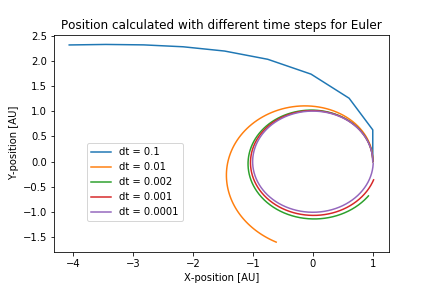
\includegraphics[width= 8.7cm]{C:/Users/Andreas/Documents/Project 5/Project-5/Data/NoClass/stabilityEuler.png}
  \caption{Stability plot of the Euler Forward method as a function of $\Delta t$.}
  \label{fig:boat1}
\end{figure}
\begin{figure}[H]  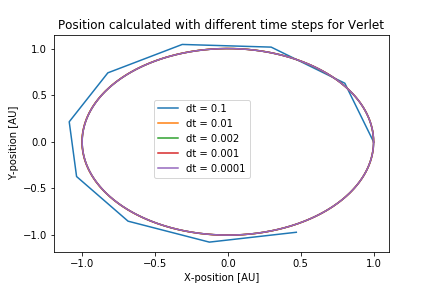
\includegraphics[width= 8.7cm]{C:/Users/Andreas/Documents/Project 5/Project-5/Data/NoClass/stabilityVerlet.png}
  \caption{Stability plot of the velocity Verlot method as a function of $\Delta t$.}
  \label{fig:boat2}
\end{figure}

\subsection{Energy}

The energy is relatily conserved taking in to account the distance is in AU and speed in AU/year. Figure 3-6 show that the changes are minimal through the year.
\begin{figure}[H]  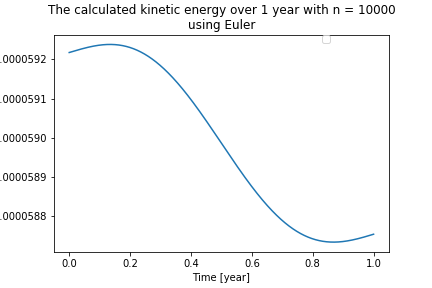
\includegraphics[width= 8.7cm]{C:/Users/Andreas/Documents/Project 5/Project-5/Data/Class/plotEulerKinetisk.png}
  \caption{The kinetic energy for the system over a year calculated using Eulrer Forward method with 10000 iterations}
  \label{fig:boat2}
\end{figure}
\begin{figure}[H]  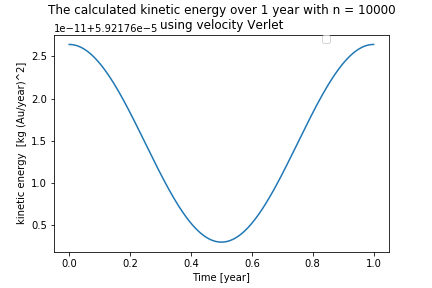
\includegraphics[width= 8.7cm]{C:/Users/Andreas/Documents/Project 5/Project-5/Data/Class/plotKinetiskVerlet.png}
  \caption{The kinetic energy for the system over a year calculated using Velocity Verlet method with 10000 iterations}
  \label{fig:boat2}
\end{figure}
\begin{figure}[H]  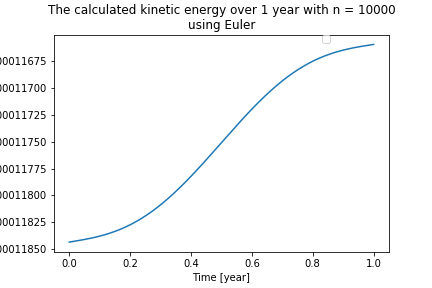
\includegraphics[width= 8.7cm]{C:/Users/Andreas/Documents/Project 5/Project-5/Data/Class/plotEulerPotensiel.png}
  \caption{The potensial energy for the system over a year calculated using Euler Forward method with 10000 iterations}
  \label{fig:boat2}
\end{figure}
\begin{figure}[H]  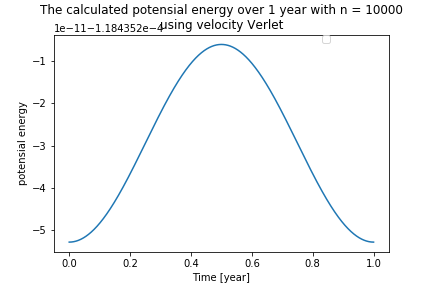
\includegraphics[width= 8.7cm]{C:/Users/Andreas/Documents/Project 5/Project-5/Data/Class/plotVerletPotensiel.png}
  \caption{The potensial energy for the system over a year calculated using Velocity Verlot method with 10000 iterations}
  \label{fig:boat2}
\end{figure}


\subsection{Escape velocity for earth}

The esacpe velocity for earth orbiting the sun was earlier found to be $v_e = 2\pi \sqrt{2} (AU/year)$ and looking at Figure 7 this is close to $V = 2.82\pi$ which also seem to escape the orbit of the sun.
\begin{figure}[H]  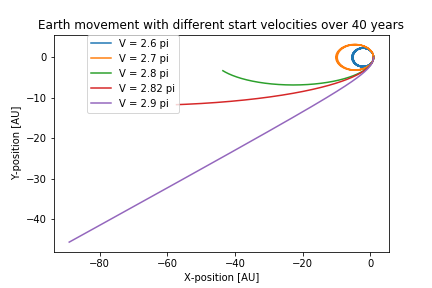
\includegraphics[width= 8.7cm]{C:/Users/Andreas/Documents/Project 5/Project-5/Data/NoClass/velocityEscape40.png}
  \caption{Plot of Earth orbit with different start veloceties (V. The plot is over a period of 40 years.}
  \label{fig:boat2}
\end{figure}

\section{Conclusion}

%----------------------------------------------------------------------------------------
%	REFERENCE LIST
%----------------------------------------------------------------------------------------

\begin{thebibliography}{99} % Bibliography - this is intentionally simple in this template
%A statement requiring citation \cite{Hjorth-Jensen:2015dg}.
\bibitem[Hjorth-Jensen, 2015]{Hjorth-Jensen:2015dg}
Hjort-Jensen, M. (2015).
\newblock Computational Physics.
\bibitem[Hjorth-Jensen]{Hjorth-Jensen}
Hjort-Jensen, M.
\newblock https://github.com/CompPhysics/ComputationalPhysics

 
\end{thebibliography}

%----------------------------------------------------------------------------------------

\end{document}
